%\documentstyle[a4j,epsbox,graphicx]{jarticle}
\documentclass[a4j]{jarticle}%変更禁止!
%%%%%%%%%%%%usepackageは適宜追加してください.%%%%%%%%%%%%%%%%%%%%%%%%%%%%%%%%%%%%%%%%%%%%%%%%%%%
%\usepackage{epsbox}
%\usepackage{graphicx}
\usepackage[dvipdfmx]{graphicx,color}
%%%%%%%%%%%%%%%%%%%%%%%%%%%ここから変更禁止%%%%%%%%%%%%%%%%%%%%%%%%%%%%%%%%%%%%%%%%%%%%%%%%%%
\topmargin -28mm
\oddsidemargin -15mm
\evensidemargin -15mm
\textwidth 185mm
\textheight 275mm
\columnsep 6mm

%\def\toujitu{Dec. 2019}

\makeatletter
\def\section{\@startsection{section}{2}{\z@}{.8ex plus .8ex minus
 .2ex}{.05ex plus .07ex}{\large\bf}}
\makeatother
\makeatletter
\def\subsection{\@startsection{subsection}{2}{\z@}{.8ex plus .8ex minus
 .2ex}{.05ex plus .07ex}{\bf}}
\makeatother


\pagestyle{empty}

\begin{document}

\baselineskip 4.75mm

\twocolumn
[
\footnotesize
\begin{center}
{~}\\
%\begin{center}
%{ユビキタスウェアラブルワークショップ2019 
%\hfill \toujitu}\\
%%%%%%%%%%%%%%%%%%%%%%%%%%%ここまで変更禁止%%%%%%%%%%%%%%%%%%%%%%%%%%%%%%%%%%%%%%%%%%%%%%%%%%

%%%注意!!\vspaceは図表部分のみ見にくく(醜く)ならない範囲内で使用可能とします.%%%%%%%%%%%%%%%%%%%%%%%%%%%%

\medskip
{\large
%タイトル
{\bf 圧力センサ搭載ヘルメットを用いた個人識別手法の提案}\\
}
\medskip
{\large
%著者 同じ所属の人が連続する場合は連続する同じ所属の著者の最後の著者のみに所属を付けること.
         藤井敦寛(立命館大学),村尾和哉(立命館大学,JSTさきがけ)
}
\end{center}
]

\section{はじめに}
近年販売されている四輪車の多くはスマートキーシステムを導入している.スマートキーシステムは電子キーをポケットなどに入れて接近すると,それを感知しドアの施錠,解錠やエンジンの始動をボタン一つで操作できるようにする機能である.このシステムは二輪車においても導入されつつある.二輪車におけるスマートキーシステムも同様に,電子キーを所持しておくことで,キーシリンダーにキーを挿し込む手間なくラゲッジスペース(メットイン)の解錠やエンジンの始動が可能になるという機能である.しかしながら,このシステムはキーを所持しておかなければならず,鍵の紛失の恐れ,更には鍵の盗難による車両盗難のリスクがある.
本研究では,圧力センサを搭載したヘルメットを装着することで,頭部形状に基づき個人識別をする手法を提案する.二輪車での走行で必要であるヘルメットを用いた本人認証が実現できれば,既存のキーの問題点を解決できると考えた.予め車両とリンクしてあるヘルメットをキーの代わりとして,二輪車のヘルメットロックに装備しておく.すると,利用者は身体一つで乗車できるため,鍵の紛失のリスクを減少させることができる.そして,利用者はヘルメットを被ることで認証を行う.車両の持ち主がヘルメットを被った場合はエンジンの始動を可能にする.その一方で,車両の持ち主以外がヘルメットを被った場合はエンジンの始動ができないような機能を実現することで,車両盗難のリスクを減少させることができる.
以降,2章では関連研究を紹介する.3章では提案手法について述べ,4章では提案手法の精度を評価し,最後に5章で本研究をまとめる.

\section{関連研究}
提案手法は,ヘルメットを装着した際に取得できる,装着者の頭部形状を用いて個人を識別する.識別に用いる要素は個人の特徴が存在し,複製が難しいものが適している.白川らは虹彩と目の周辺画像を統合して認証する手法\cite{iris_eye}を提案しているが,目の前にカメラを設置する必要があり,ヘルメットに取り付けると視界を遮るおそれがある.頭部形状は視界を遮ることなく取得できる.また,頭部形状に個人差が存在しており,かつ複製が難しいため,個人識別に適していると考えられる.

メガネ型デバイスを用いた経皮水分蒸散量の常時測定システム\cite{glasses}やHappyMouth:マスク型デバイスによる対面コミュニケーション能力の拡張\cite{happymouth}のように,顔に取り付けるウェアラブルデバイスは多数研究されているが,頭部装着型デバイスとしては,新島らの導電性高分子電極を用いた帽子型筋電センサの提案\cite{cap_sensor}のみであり,中でもウェアラブルデバイスとしてヘルメットを用いた先行研究は存在しない.

越前らが写真からの指紋復元の脅威とその対策技術\cite{finger_print}を提案しているように,指紋認証には複製の恐れがある.しかも,少ない写真などで簡易に複製が可能である.その一方で,頭部形状の複製は用意ではない.立体形状が正確でないと認証が突破できない.そのため,写真から複製するにはかなりの枚数が必要になると考えられる.また,複製物の大きさは頭部サイズであるため,かなり大掛かりになる.

雨坂らの外耳道伝達関数を用いた頭部状態認識手法\cite{head_from_ear}をはじめとして,表情などの頭部状態を認識する研究は数多くあるが,頭部状態の中でも頭部の形状を認識する先行研究は存在しない.

当麻らのステレオカメラを用いた顔認証システム\cite{face}など,顔認証の技術は研究され続けている.カメラを車両に取り付けることで,顔認証システムを実装することは可能であるが,二輪車においては屋外での悪天候下における使用,耐久性も考慮しなければならず,カメラの使用は向かないだろう.⇒虹彩認証も駄目というくだりへ続く

\section{提案手法}
本章では提案手法の詳細を述べる.本研究はヘルメットをキーの代わりとして用いるために,圧力センサを搭載したヘルメットを装着し,装着者の頭部形状を取得することで個人識別を行う手法を提案する.本手法では個人識別を行うために,着座状態でヘルメットを装着している環境を想定している.

\subsection{ハードウェアの実装}
提案手法に用いる,圧力センサを搭載したヘルメットを実装した.このプロトタイプデバイスの全体図を図\ref{met_over},ヘルメット内部を図\ref{met_in}に示す.センサ値を正しく取得するには,センサとヘルメット装着者の頭部が密着している必要がある.そのため,フルフェイス型のB\&B社製BB100フルフェイスヘルメットを用いた.ヘルメット内部にはインターリンク エレクトロニクス社製の圧力センサFSR402,FSR402 ShortTailを取り付けた.圧力センサは頭頂部に4個,頭頂部周囲に16個,後頭部に6個,左右チークパッド部に6個の合計32個を搭載した.
各圧力センサはヘルメット外部に取り付けた10KΩの抵抗を配線してあるプリント基板を経由して,Arduino MEGA2560 R3のアナログ入力ポートに接続した.このプリント基板を図\ref{print}に示す.また,回路図は図\ref{circuit}である.
図\ref{device}の右図はヘルメット内部の様子である.今回用いたヘルメットはフリーサイズであり,また内装の脱着が困難であった.そのため,頭頂部の内装を取り外して,新たに厚みのあるウレタンスポンジを取り付けた.図\ref{sensor}のように,取り付けたウレタンスポンジの中央部に切り込みを入れ,圧力センサを挿し込んだ.

\subsection{識別手法}
ユーザはヘルメットを被った状態で2秒静止し,32個の圧力センサの電圧値を取得する.各センサごとに2秒間の平均値を計算し32次元のベクトルを作成する.ユーザは最初に本人のデータとして複数サンプルのデータを登録する.識別時は登録データ群と未知のユーザの圧力データのマハラノビス距離を計算する.この距離が閾値未満となった場合本人として認証し,閾値以上となった場合は他人として拒否する.

\section{評価}
提案手法の有効性を確認するために,被験者5名(A$\sim$E,全員男性,平均年齢22歳)にプロトタイプデバイスを着用させ,サンプリングレート約30Hzでセンサデータを収集した.2秒間着用して取り外し,再び着用する試行を1セットとして合計10セット(2秒$\times$20回分)を収集した.データ収集は1人当たり1日最大4セットとし,複数日に渡って実施した.センサと頭部のさまざまな位置関係のデータを採取するために,セット間に30分以上の休憩時間を設けた.\par
収集したすべてのデータに対して主成分分析を行い,2次元に圧縮したデータを2次元平面上にプロットした結果を図\ref{pca}に示す.図より,装着位置のずれによって同一被験者のデータ群にばらつきはあるが,被験者のデータ群どうしの重なりが小さいことから,ヘルメット内部に搭載した圧力センサのデータから装着者を識別できると考える.\par

\section{まとめ}
本研究では,圧力センサを内部に取り付けたヘルメットを着用することで頭部の形状を計測し,頭部形状の個人差から二輪車の所有者本人を識別する手法を提案した.評価実験の結果より,個人間にデータのばらつきがあり,個人を高精度で識別できそうであることを確認した.今後は,被験者を増やしてデータを収集し,実環境で提案手法の評価をする.また,提案手法の利用者のデータ群に差がないときの個人識別方法を定義する.

\begin{figure}[!t]
  \begin{center}
    \includegraphics[width=1\linewidth]{met_over.eps}
  \end{center}
    \vspace{-8mm}
  \caption{プロトタイプデバイスの全体図}
  \label{met_over}
\end{figure}

\begin{figure}[!t]
  \begin{center}
    \includegraphics[width=1\linewidth]{met_in.eps}
  \end{center}
    \vspace{-8mm}
  \caption{ヘルメットの内部}
  \label{met_in}
\end{figure}

\begin{figure}[!t]
  \begin{center}
    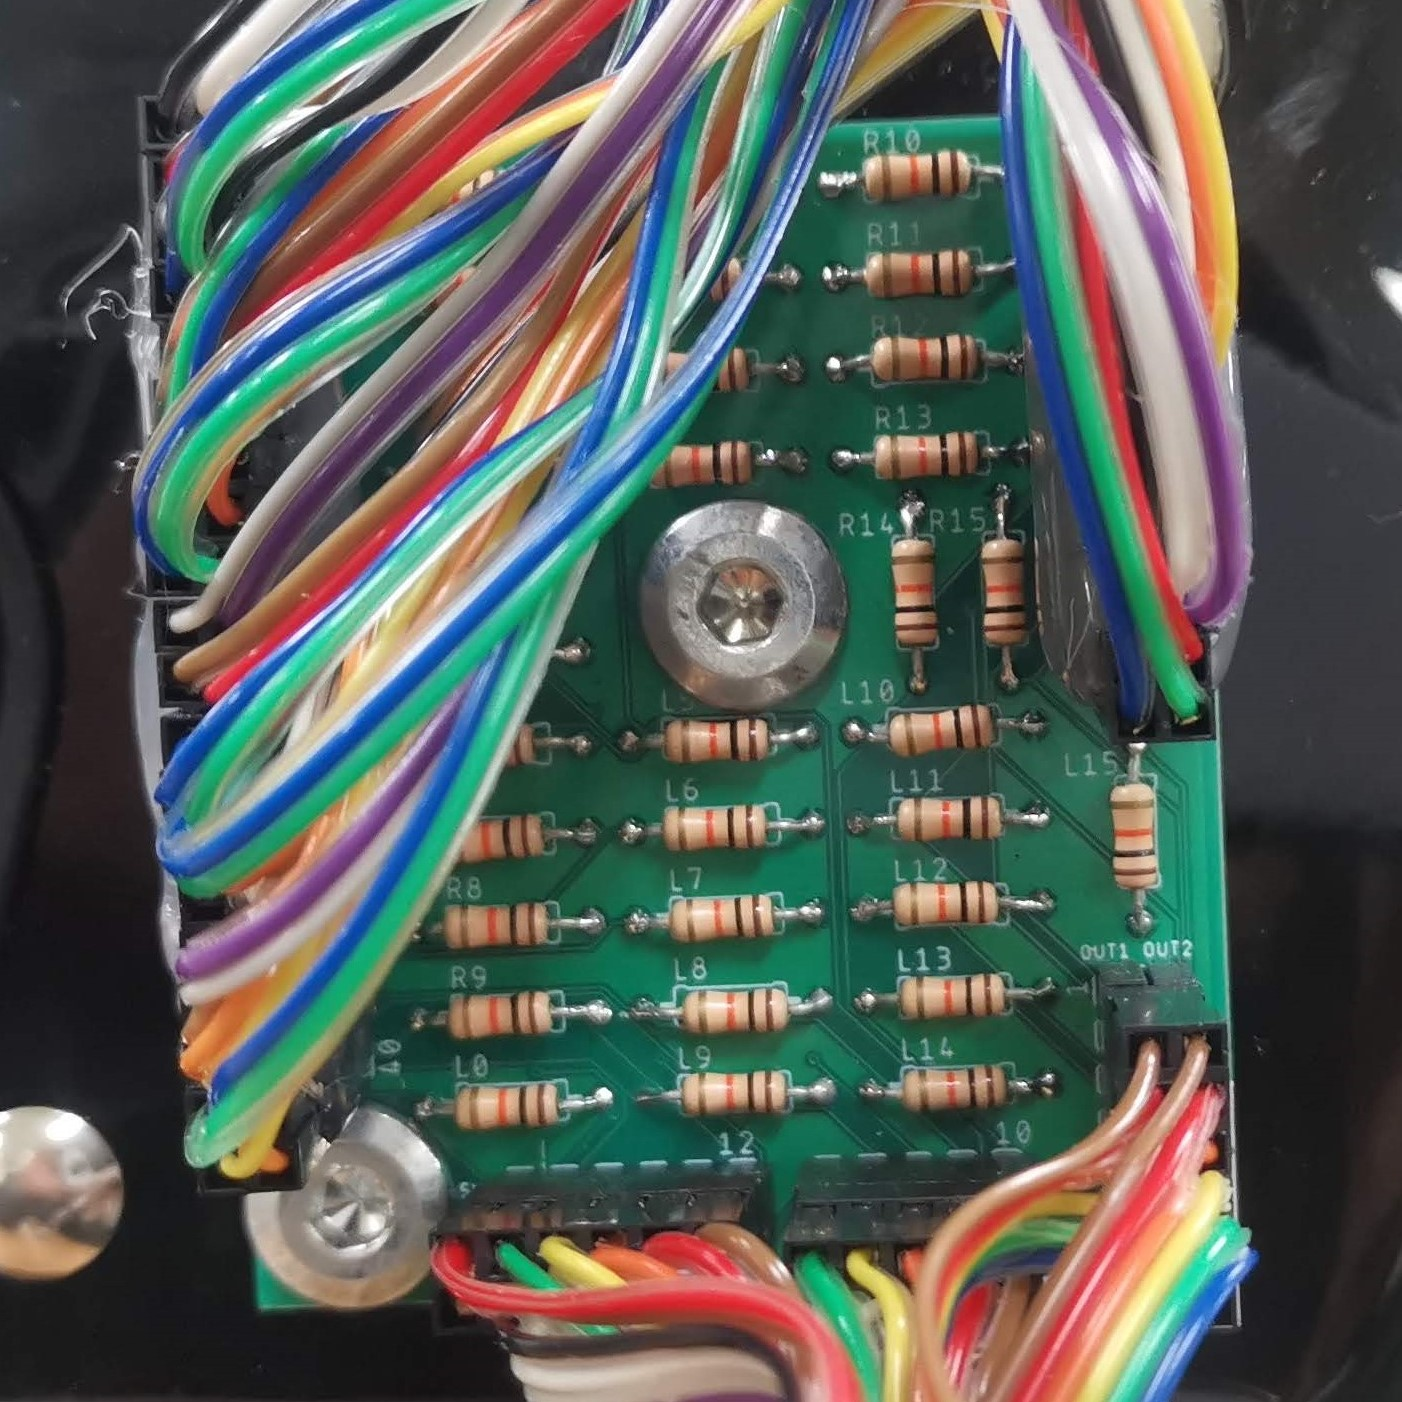
\includegraphics[width=1\linewidth]{print.eps}
  \end{center}
    \vspace{-8mm}
  \caption{プリント基板}
  \label{print}
\end{figure}

\begin{figure}[!t]
  \begin{center}
    \includegraphics[width=1\linewidth]{circuit.eps}
  \end{center}
    \vspace{-8mm}
  \caption{プリント基板の回路図}
  \label{circuit}
\end{figure}

\begin{figure}[!t]
  \begin{center}
    \includegraphics[width=1\linewidth]{sensor.eps}
  \end{center}
    \vspace{-8mm}
  \caption{センサの装着方法}
  \label{sensor}
\end{figure}

\begin{figure}[!t]
  \begin{center}
    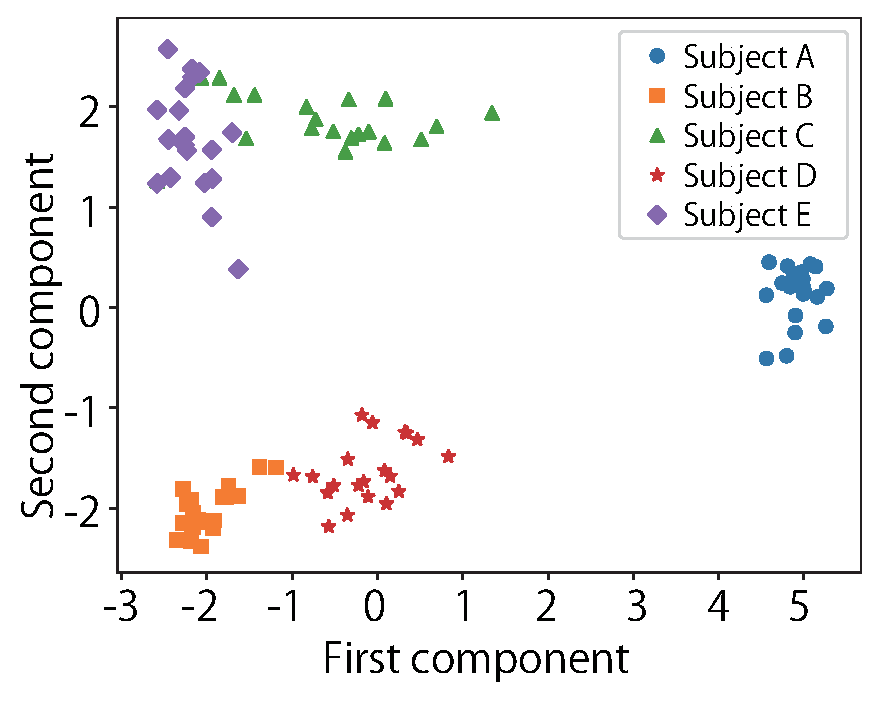
\includegraphics[width=1\linewidth]{PCA.eps}
  \end{center}
    \vspace{-8mm}
  \caption{PCAによる分析結果}
  \label{pca}
\end{figure}

\bibliography{../references}
\bibliographystyle{junsrt}

\end{document}
